\documentclass[portrait,a1paper,fontscale=0.45]{kuleuvenposter}
%\documentclass[landscape,a1paper,fontscale=0.45]{kuleuvenposter}
%,paperheight=24in,paperwidth=36in%
%,fontscale=0.467
\usepackage{color}
\usepackage{amsmath}
\usepackage{amsthm}
\usepackage{amsfonts}
\usepackage{enumitem}
\usepackage{geometry}
\usepackage{caption}
\usepackage{subfigure}
\usepackage{tikz}
\usetikzlibrary{calc,shapes,backgrounds,fit,arrows.meta,positioning,decorations.pathmorphing}
\usepackage{pgfplots}

\usepackage{mathtools}
\mathtoolsset{showonlyrefs}
\usepackage{csvsimple}
%
\def\stepwidth{7}
\def\stepheight{5}
\def\N{3}
\pgfmathtruncatemacro\Nm{\N-1} 
%
\tikzset{encircle/.style={ellipse,minimum width=1.2cm, minimum height=0.7cm, draw=KULeuvenRechtsgeleerdheid,line width=2pt}}
\tikzset{hllabel/.style={KULeuvenRechtsgeleerdheid,font=\fontsize{10}{10}\ttfamily,text width=.5*\stepwidth cm}}
\tikzset{hlnode/.style={KULeuvenRechtsgeleerdheid,font=\fontsize{10}{10}\ttfamily,text width=.5*\stepwidth cm}}
\tikzset{hlline/.style={draw=KULeuvenRechtsgeleerdheid, line width=2pt, shorten >=2pt, shorten <=2pt}}
% For the various arrows to be used
\tikzset{
coarse/.style={KULeuvenBlauw,{Triangle Cap[reversed]}-{Triangle Cap[]},shorten <=5pt,shorten >=5pt,line width=1.2em},
fine/.style={KULeuvenBlauw,{Triangle Cap[reversed]}-{Triangle Cap[]},shorten <=5pt,shorten >=5pt,line width=1.2em},
noisy/.style={KULeuvenBlauw,{Triangle Cap[reversed]}-{Triangle Cap[]},shorten <=5pt,shorten >=5pt,line width=1.2em},
restriction/.style={KULeuvenLichtblauw,{Triangle Cap[cap angle=120, reversed]}-{Triangle Cap[cap angle=120]},shorten <=5pt,shorten >=2pt,line width=1.2em},
matchingfrommicro/.style={KULeuvenLichtblauw,{Triangle Cap[cap angle=120, reversed]}-{Butt Cap},shorten <=2pt,line width=.4em},
matchingfrommacro/.style={KULeuvenLichtblauw,{Triangle Cap[cap angle=120, reversed]}-{Butt Cap},shorten <=0pt,line width=.8em},
matching/.style={KULeuvenLichtblauw,-{Triangle Cap[cap angle=120]},shorten >=2pt,line width=1.2em},
microcopy/.style={black!5,-,shorten >=2pt,shorten <=2pt,line width=.4em},
macrocopy/.style={KULeuvenLichtblauw,-,shorten >=2pt,shorten <=2pt,line width=.8em}
}
%
\makeatletter
\g@addto@macro\normalsize{%
  \setlength\abovedisplayskip{5pt}
  \setlength\belowdisplayskip{3pt}
  \setlength\abovedisplayshortskip{0pt}
  \setlength\belowdisplayshortskip{0pt}
}
\makeatother

\newcommand{\dd}{\,\mathrm{d}}
\newcommand{\half}{\frac{1}{2}}
\newcommand\eff{\mbox{eff}}

\setlength{\columnsep}{0.7em}
\setlength{\columnseprule}{0mm}

%\setlength{\parskip}{0pt}
\begin{document}

\begin{poster}{columns=4,Faculteit=Ingenieurswetenschappen} 
{ % the formatting is done here, as the desired font size will depend on the title length
\spaceskip=1\fontdimen2\font plus 1\fontdimen3\font minus \fontdimen4\font % Make larger spaced in the title 
  \Huge\bfseries Parareal computation of SDEs with time-scale separation
}
{ % Names (and subtitle) go(es) here
  Fr\'ed\'eric Legoll\textsuperscript{1},Tony Leli\`evre\textsuperscript{1}, \underline{Keith Myerscough}\textsuperscript{2} and Giovanni Samaey\textsuperscript{2}\\
  {\footnotesize \textsuperscript{1}Ecole des Ponts ParisTech, \textsuperscript{2}KU Leuven}}
{ % Personal images (photo/QR code to website
  
\includegraphics[width=\footerheight]{specific/qrcode}%
  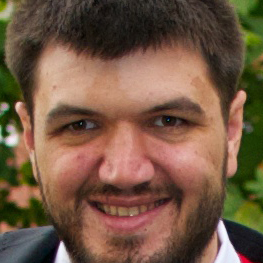
\includegraphics[width=\footerheight]{specific/photo.jpg}
}
{ % Personal details
  Keith Myerscough\\{\texttt keith.myerscough@kuleuven.be}\\people.cs.kuleuven.be/\~{}keith.myerscough/
}
{% Text to state association
In association with:%
}
{% Logo's of associated institutes/universities/companies/funding etc.
  
\includegraphics[height=.8\footerheight]{specific/logo_EcolePonts} % 
}
{ % Department name
  Department of Computer Science%
}
{ % Department logo
  
\includegraphics[height=\footerheight]{images/logo_CS}% 
}

%
\begin{posterbox}%
[name=micro-macro modelling, column=0, row=0, boxColorOne=KULeuvenFaculteit!15!white, borderColor=KULeuvenFaculteit]%
%[name=micro-macro modelling, column=0, row=0, boxColorOne=KULeuvenFaculteit!15!white, textborder=open, borderColor=KULeuvenFaculteit, headerColorOne=KULeuvenFaculteit, headerborder=open, headerBorderColor=KULeuvenFaculteit,  headerFontColor=white]%
%{Micro-macro modelling}%
{In a nutshell}%
%\begin{noindentitemize}
%\item The microscopic system is governed by known equations of motion, which we consider `exact'
%\item From the microscopic state we can extract macroscopic quantities
%\item We assume we have some (possibly inaccurate) model for the evolution of the macroscopic variables
%\item Observables of interest are defined as functions of the macroscopic state
%\end{noindentitemize}
\begin{description}
\item[Goal] Simulate slow-fast SDEs over long time, quickly
\item[Model] Slow-fast system of SDEs, and a macroscopic model taken from the ``fast'' limit
\item[Method] Parallel-in-time algorithm that iteratively improves the macroscopic result
\item[Result] Reduction in wall clock time
\item[Bonus] Lower variance than full microscopic model
\end{description}
\end{posterbox}

\begin{posterbox}[name=microscopic, column=0,below=micro-macro modelling]{Microscopic model}
\begin{noindentitemize}
%\item We study as the microscopic system a slow-fast system of coupled SDEs
\item Slow-fast system of coupled SDEs
\begin{align}
\dd X &= (-X_t^3 + X_t + Y_t^2) \dd t + \sqrt{\frac{2}{\beta}} \dd B_t^{(x)}  \label{eq:xParisdyn}\\
\dd Y &= \frac{1}{\epsilon}(X_t - Y_t) \dd t + \sqrt{\frac{2}{\beta\epsilon}} \dd B_t^{(y)}. \label{eq:yParisdyn}
\end{align}
%
%\item Modeled as an ensemble $\mathcal{X}_t = \lbrace X_t^p,Y_t^p,W_t^p \rbrace_{p=1}^P$ of particles with weight $W^p$
\item Modeled as an ensemble $\mathcal{X}_t$ of particles with positions ($X_t^p$, $Y_t^p$) and weight $W^p$
\item Time integrator: a Lie-Trotter splitting, updating $X_t$ first, then $Y_t$
\item Validation: \emph{deterministic} solution given by the Fokker-Planck equation, akin to the macroscopic model
\end{noindentitemize}
\end{posterbox}

\begin{posterbox}%
[name=parareal micro-macro, column=1, above=bottom, boxColorOne=KULeuvenFaculteit!15!white, borderColor=KULeuvenFaculteit]%
{The parareal algorithm}
%\begin{noindentitemize}
%\item The parareal algorith iteratively improves the macroscopic propagator, by computing the discrepancies between the macroscopic and the microscopic models \emph{in parallel}
%\item By employing the microscopic propagator only in parallel, there is a reduction in \emph{wall clock time} if there are fewer iterations needed than time steps
%\item The error is dominated by variance (see figures $\rightarrow$)%the variance due to the stochastic nature of the microscopic propagator
%\item This variance is greatly reduced by using a particle propagator with {\color{KULeuvenSecundair}correlated noise} for the macroscopic model in computing the discrepancies between the models
%\end{noindentitemize}
\begin{description}
\item[Iteratively improves] the macroscopic propagator by computing the discrepancies between the {\color{KULeuvenBlauw}macroscopic} and the {\color{KULeuvenFaculteit}microscopic} models \emph{in parallel}
\item[Parallel] use of the microscopic propagator gives a reduction in \emph{wall clock time} if there are fewer iterations needed than time steps
\item[Variance] of the stochastic microscopic propagator dominates the error (see figures $\rightarrow$)%the variance due to the stochastic nature of the microscopic propagator
\item[Reduction in variance] by using a particle propagator with {\color{KULeuvenSecundair}correlated noise} for the macroscopic model in computing the discrepancies between the models
\end{description}
%\documentclass[tikz]{standalone}
%\usepackage{pgfmath}
%\usepackage{csvsimple}
%\usetikzlibrary{calc,arrows.meta}
%
%\begin{document}
\newlength{\intervalwidth}
\newlength{\controldistance}
\newlength{\yscale}
\setlength\intervalwidth{1cm}
\setlength\controldistance{.3cm}
\setlength\yscale{.4cm}
\def\tikzscale{0.80}
\pgfmathsetmacro\invtikzscale{1/\tikzscale}

% A simple empty decoration, that is used to ignore the last bit of the path
\pgfdeclaredecoration{ignore}{final}
{
\state{final}{}
}

% Declare the actual decoration.
\pgfdeclaremetadecoration{begin}{initial}{
    \state{initial}[
        width={\the\pgfdecorationsegmentlength},
        next state=final
    ]
    {\decoration{curveto}}

    \state{final}
    {\decoration{ignore}}
}

% Create a key for easy access to the decoration (as suggested by Jake).
\tikzset{begin segment/.style={decoration={begin},decorate, segment length=#1}}

{\normalsize
\begin{center}
\resizebox{0.8\textwidth}{!}{%
\begin{tikzpicture}
  \foreach\k in {0} {
  \pgfmathtruncatemacro\knext{\k+1}
  \useasboundingbox (-1em,1.25\yscale) rectangle (4.0\intervalwidth,8.5\yscale);
  \begin{scope}
  \clip (-1em,1.25\yscale) rectangle (3.5\intervalwidth,8.5\yscale);
  %\draw[xstep=\intervalwidth,ystep=\yscale] (0,0) grid (4\intervalwidth,8\yscale);

  \ifthenelse{\k = 0}{%
    \tikzset{rho/.style={shape=circle,inner sep=1pt,draw=KULeuvenBlauw,fill=KULeuvenBlauw}}
    \tikzset{rhobar/.style={shape=circle,inner sep=1pt,draw=KULeuvenBlauw,fill=white}}
    \tikzset{phi/.style={shape=circle,inner sep=1pt,draw=KULeuvenSecundair}}
    \tikzset{mu/.style={shape=circle,inner sep=1pt,draw=KULeuvenFaculteit,fill=white}}
    \tikzset{rholine/.style={KULeuvenBlauw,dashed,line width=1pt}}
    \tikzset{philine/.style={KULeuvenSecundair,line width=1pt}}
    \tikzset{muline/.style={KULeuvenFaculteit,line width=1pt}}
    \tikzset{jumpline/.style={black,|->,line width=1pt}}
  }{%
    \tikzset{rho/.style={shape=coordinate,inner sep=0pt,draw=KULeuvenBlauw,fill=KULeuvenBlauw}}
    \tikzset{rhobar/.style={shape=coordinate,inner sep=0pt,draw=KULeuvenBlauw,fill=white}}
    \tikzset{phi/.style={shape=coordinate,inner sep=0pt,draw=KULeuvenSecundair}}
    \tikzset{mu/.style={shape=coordinate,inner sep=0pt,draw=KULeuvenFaculteit,fill=white}}
    \tikzset{rholine/.style={begin segment=0.85\intervalwidth,KULeuvenBlauw,dashed,line width=0pt}}
    \tikzset{philine/.style={begin segment=0.75\intervalwidth,KULeuvenSecundair,line width=1pt}}
    \tikzset{muline/.style={begin segment=0.75\intervalwidth,KULeuvenFaculteit,line width=1pt}}
    \tikzset{jumpline/.style={black,|->,line width=1pt}}
  }

  \csvreader[head to column names]{specific/input.csv}
  {rho\k=\nrho,rho\k out=\nrhoout,phi\k=\nphi,phi\k in=\nphiin,%
  mu\k =\nmu,mu\k out=\nmuout,mu\k in=\nmuin,rho\knext=\nprho,rho\knext out=\nprhoout,rho\knext bar=\nprhobar,rho\knext barin=\nprhobarin}%
  {%
\pgfmathtruncatemacro\nnext{\thecsvrow}
\pgfmathtruncatemacro\n{\nnext-1}
\pgfmathtruncatemacro\nprev{\n-1}
\coordinate (rho\n) at (\n\intervalwidth, \nrho\yscale);
\coordinate (out rho\n) at (\n\intervalwidth + \controldistance, \nrho\yscale + \nrhoout\yscale);

\coordinate (phi\n) at (\n\intervalwidth, \nphi\yscale);
\coordinate (in  phi\n) at (\n\intervalwidth - \controldistance, \nphi\yscale - \nphiin\yscale);

\coordinate (mu\n) at (\n\intervalwidth, \nmu\yscale);
\coordinate (out mu\n) at (\n\intervalwidth + \controldistance, \nrho\yscale + \nmuout\yscale);
\coordinate (in  mu\n) at (\n\intervalwidth - \controldistance, \nmu\yscale  - \nmuin\yscale);

\coordinate (prho\n) at (\n\intervalwidth, \nprho\yscale);
\coordinate (out prho\n) at (\n\intervalwidth + \controldistance, \nprho\yscale + \nprhoout\yscale);
\coordinate (prhobar\n) at (\n\intervalwidth, \nprhobar\yscale);
\coordinate (in  prhobar\n) at (\n\intervalwidth - \controldistance, \nprhobar\yscale - \nprhobarin\yscale);

\ifthenelse{\n = 0}{}{%
  \draw [muline]  (rho\nprev) .. controls (out mu\nprev)  and (in mu\n)  .. (mu\n);
  \ifthenelse{\n > \k}{
    \draw [philine] (rho\nprev) .. controls (out rho\nprev) and (in phi\n) .. (phi\n);
    \draw [rholine]  (prho\nprev) .. controls (out prho\nprev)  and (in prhobar\n)  .. (prhobar\n);
  }{}
}
\node [rho] at (rho\n) {};
\node [phi] at (phi\n) {};
\node [mu]  at (mu\n)  {};
\node [rhobar] at (prhobar\n) {};
\node [rho] at (prho\n) {};
\ifthenelse{\k = 0}{
  \ifthenelse{\n > \k}{
    \draw [jumpline] (phi\n) -- (mu\n);
  rlet{orange}{KULeuvenLichtblauw}
    \draw [jumpline] (prhobar\n) -- (prho\n);
  }{}
}{} % end of conditional on k=0
  } % end of CSV reader
  \end{scope}
  \ifthenelse{\k = 0}{
    \tikzset{prop/.style={}}
    \node [color=KULeuvenFaculteit, above=.4\yscale of mu3]   {\footnotesize micro $\mathcal{X}$};
    \node [color=KULeuvenSecundair, below=.4\yscale of phi3]  {\footnotesize macro $\mathcal{Z}$};
    \node [color=KULeuvenBlauw,     left=.4\yscale of prhobar2] {\footnotesize macro $\rho$};
    \draw [->] (0,1.5\yscale) to node [above=.2em] {time} (3\intervalwidth,1.5\yscale);
    \draw [->] (0,1.5\yscale) to node [left=.2em,above,rotate=90] {value} (0,7\yscale);
    \node [anchor=south west] at (2.5\intervalwidth,2\yscale) {$k = \k$};
  }
} % end of foreach k
\end{tikzpicture}
%\end{document}
}
\end{center}
}

\end{posterbox}

\begin{posterbox}[name=macroscopic, column=0,below=microscopic, above=bottom]{Macroscopic model}
%\begin{posterbox}[name=macroscopic, column=1,row=0, above=parareal micro-macro]{Macroscopic model}
\begin{noindentitemize}
%\item \emph{assume} $\epsilon \rightarrow 0$, then $X_t$ ``feels'' only the conditional distribution of $Y_t$, a Gaussian centred at $X_t$ with variance $\frac{1}{\beta}$. 
\item Only slow variable, \emph{assume} the fast $Y_t$ is equilibrated and use only the expected value of the term $Y_t^2$
\begin{align}
\dd Z &= (-Z_t^3 + Z_t + Z_t^2 + \frac{1}{\beta}) \dd t + \sqrt{\frac{2}{\beta}} \dd B^{(x)}, \label{eq:zParisdyn}
\end{align}
or in potential form
\begin{align}
\dd Z &= -\partial_z V_{\eff} (Z_t) \dd t + \sqrt{\frac{2}{\beta}} \dd B^{(x)}. \label{eq:zParisdyn_pot}
\end{align}
%
\item The associated Fokker-Planck equation reads
\begin{equation}
\partial_t \rho(z) = \partial_z \left( \rho(z) \partial_z V_{\eff} \right) + \frac{1}{\beta} \partial_{zz} \rho(z).
\end{equation}
\item The macroscopic state is represented by integral quantities over a regular grid
%\begin{equation}
%\rho_i = \int_{x_i}^{x_{i+1}} \rho(z) \dd z,
%\end{equation}
%where the $x_i$ form an evenly spaced grid
\end{noindentitemize}
\end{posterbox}

%\begin{posterbox}[name=coupling,column=0,below=notset, above=bottom]{Coupling}
\begin{posterbox}[name=macroscopic, column=1,row=0, above=parareal micro-macro]{Coupling}
\begin{description}
\item[Restriction]($\mathcal{R}$, from micro to macro) sum the weights of all particles in each bin
%\begin{equation}
%%\rho_i = \sum_{\mbox{all particles $p$ in bin $i$}} W^p
%\rho_i = \sum_{\mbox{\footnotesize all particles $p$ in bin $i$}} W^p
%\end{equation}
\item[Matching]($\mathcal{M}$, from macro to micro) reweight particles from a known microstate $(\bar{X}^p, \bar{Y}^p, \bar{W}^p)$
%\begin{equation}
%%W^p = \bar{W}^p \frac{\rho_i}{\bar{\rho}_i} \mbox{ for } {\lbrace p: x_i \leq X_t^p < x_{i+1} \rbrace} \mbox{ for } i=0,1,\ldots,N-1
%W^p = \bar{W}^p \frac{\rho_i}{\bar{\rho}_i}\quad \mbox{\footnotesize for all particles $p$ in bin $i$}
%\end{equation}
\item[Resampling]($\mathcal{M}^*$, optional) retrieve an ensemble with all particles equal in weight
\end{description}
\end{posterbox}

\begin{posterbox}[name=convergenceK, column=2, below=notset, above=bottom, borderColor=KULeuvenFaculteit]{Convergence in iterations}%the number of iterations}
\begin{tikzpicture}
\node (inK) {
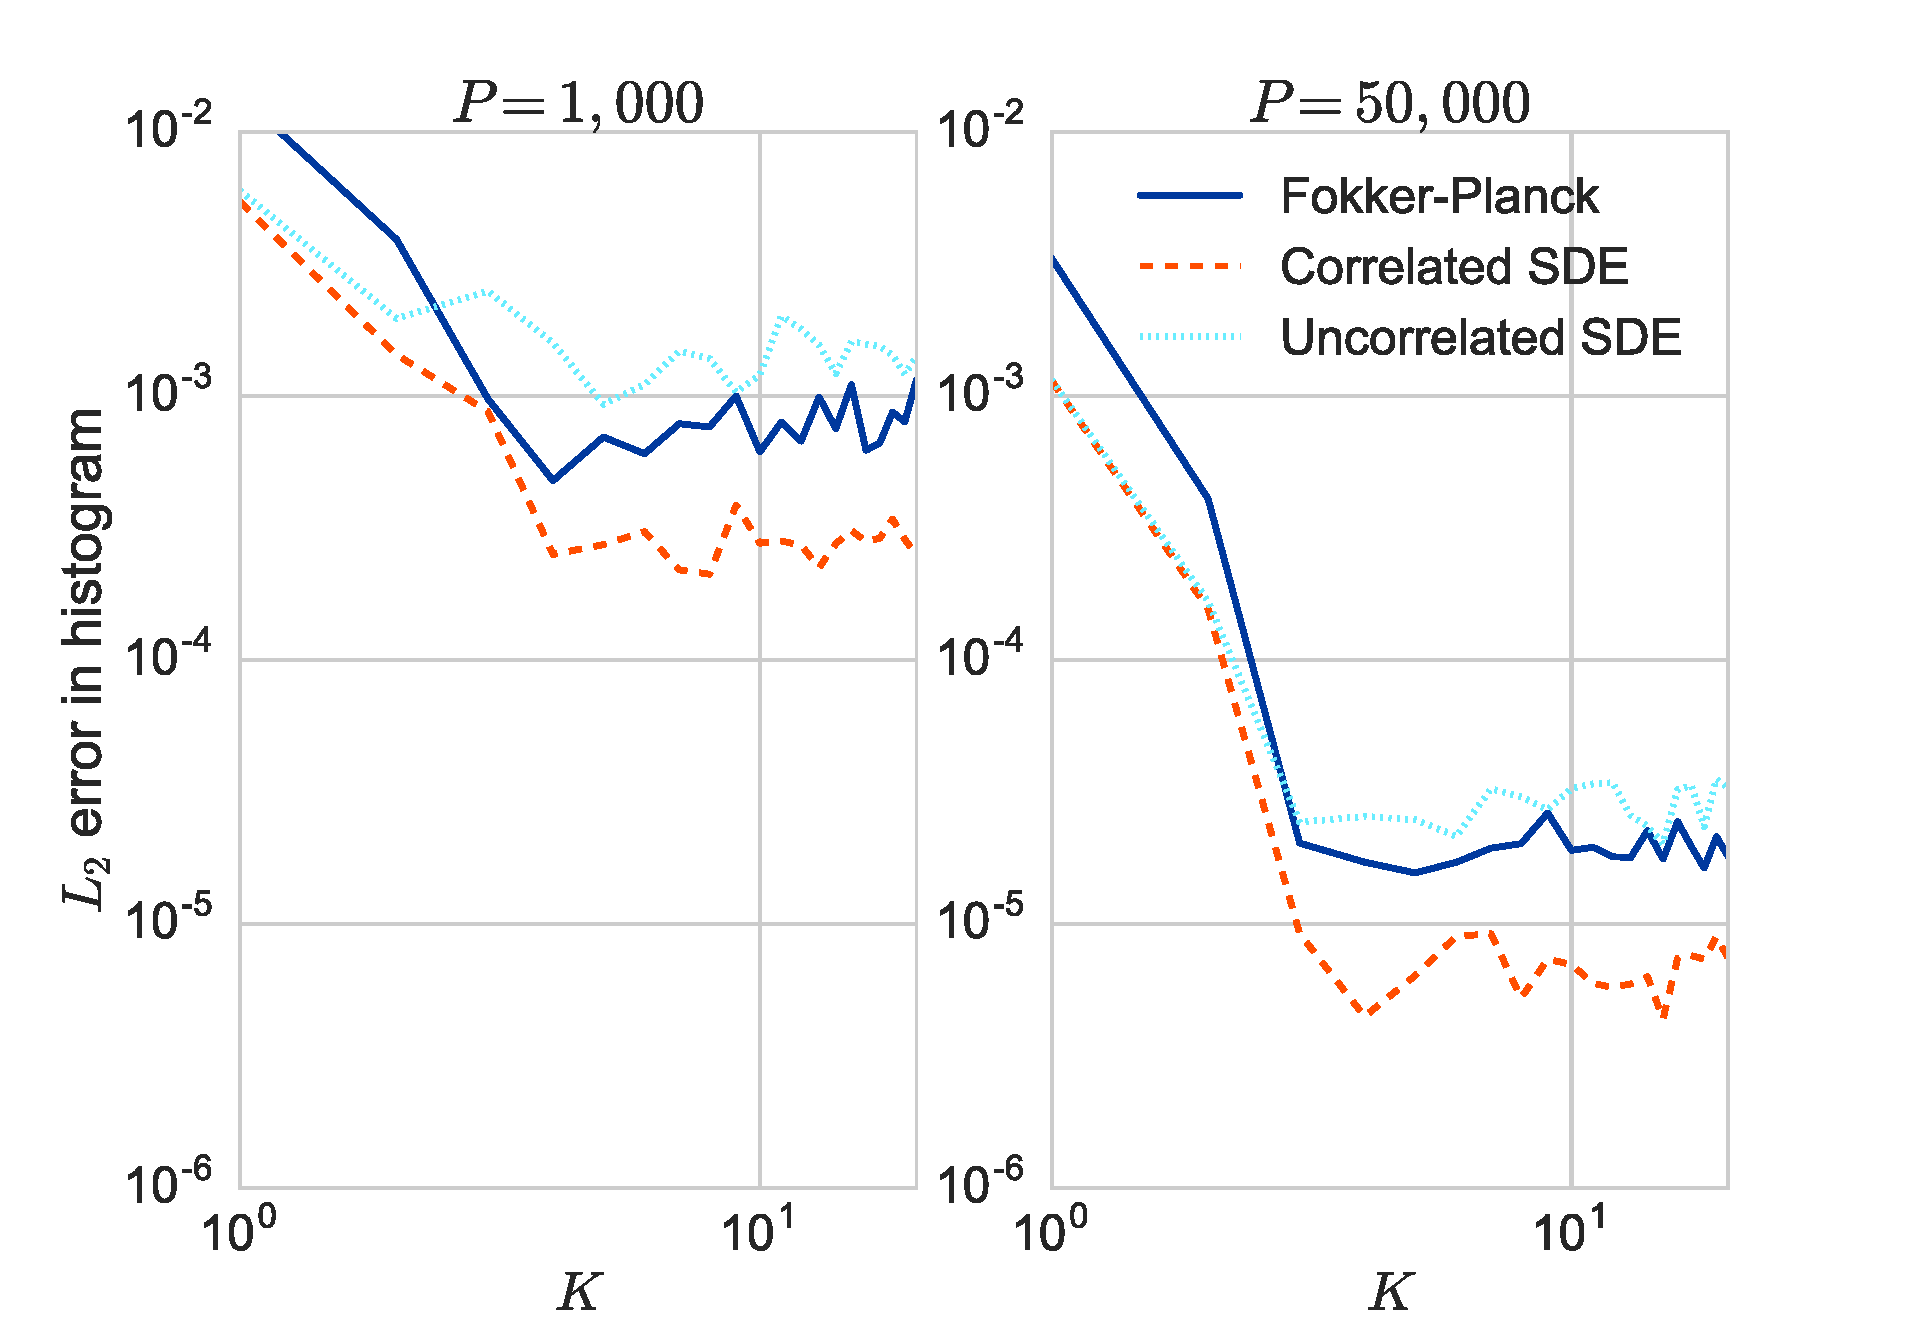
\includegraphics[width=\textwidth]{specific/inK}
};
\node [hlnode, anchor=south west] (inKlabel) at ($(inK.south west)!.1!(inK.north east)$) {Iteration converges in a few steps, need only K/N of serial wall clock time};
\end{tikzpicture}
\end{posterbox}

\begin{posterbox}[name=convergenceP, column=3, below=notset, above=bottom, borderColor=KULeuvenFaculteit]{Convergence in number of particles}%the number of particles}
\begin{tikzpicture}
\node (invalue) {
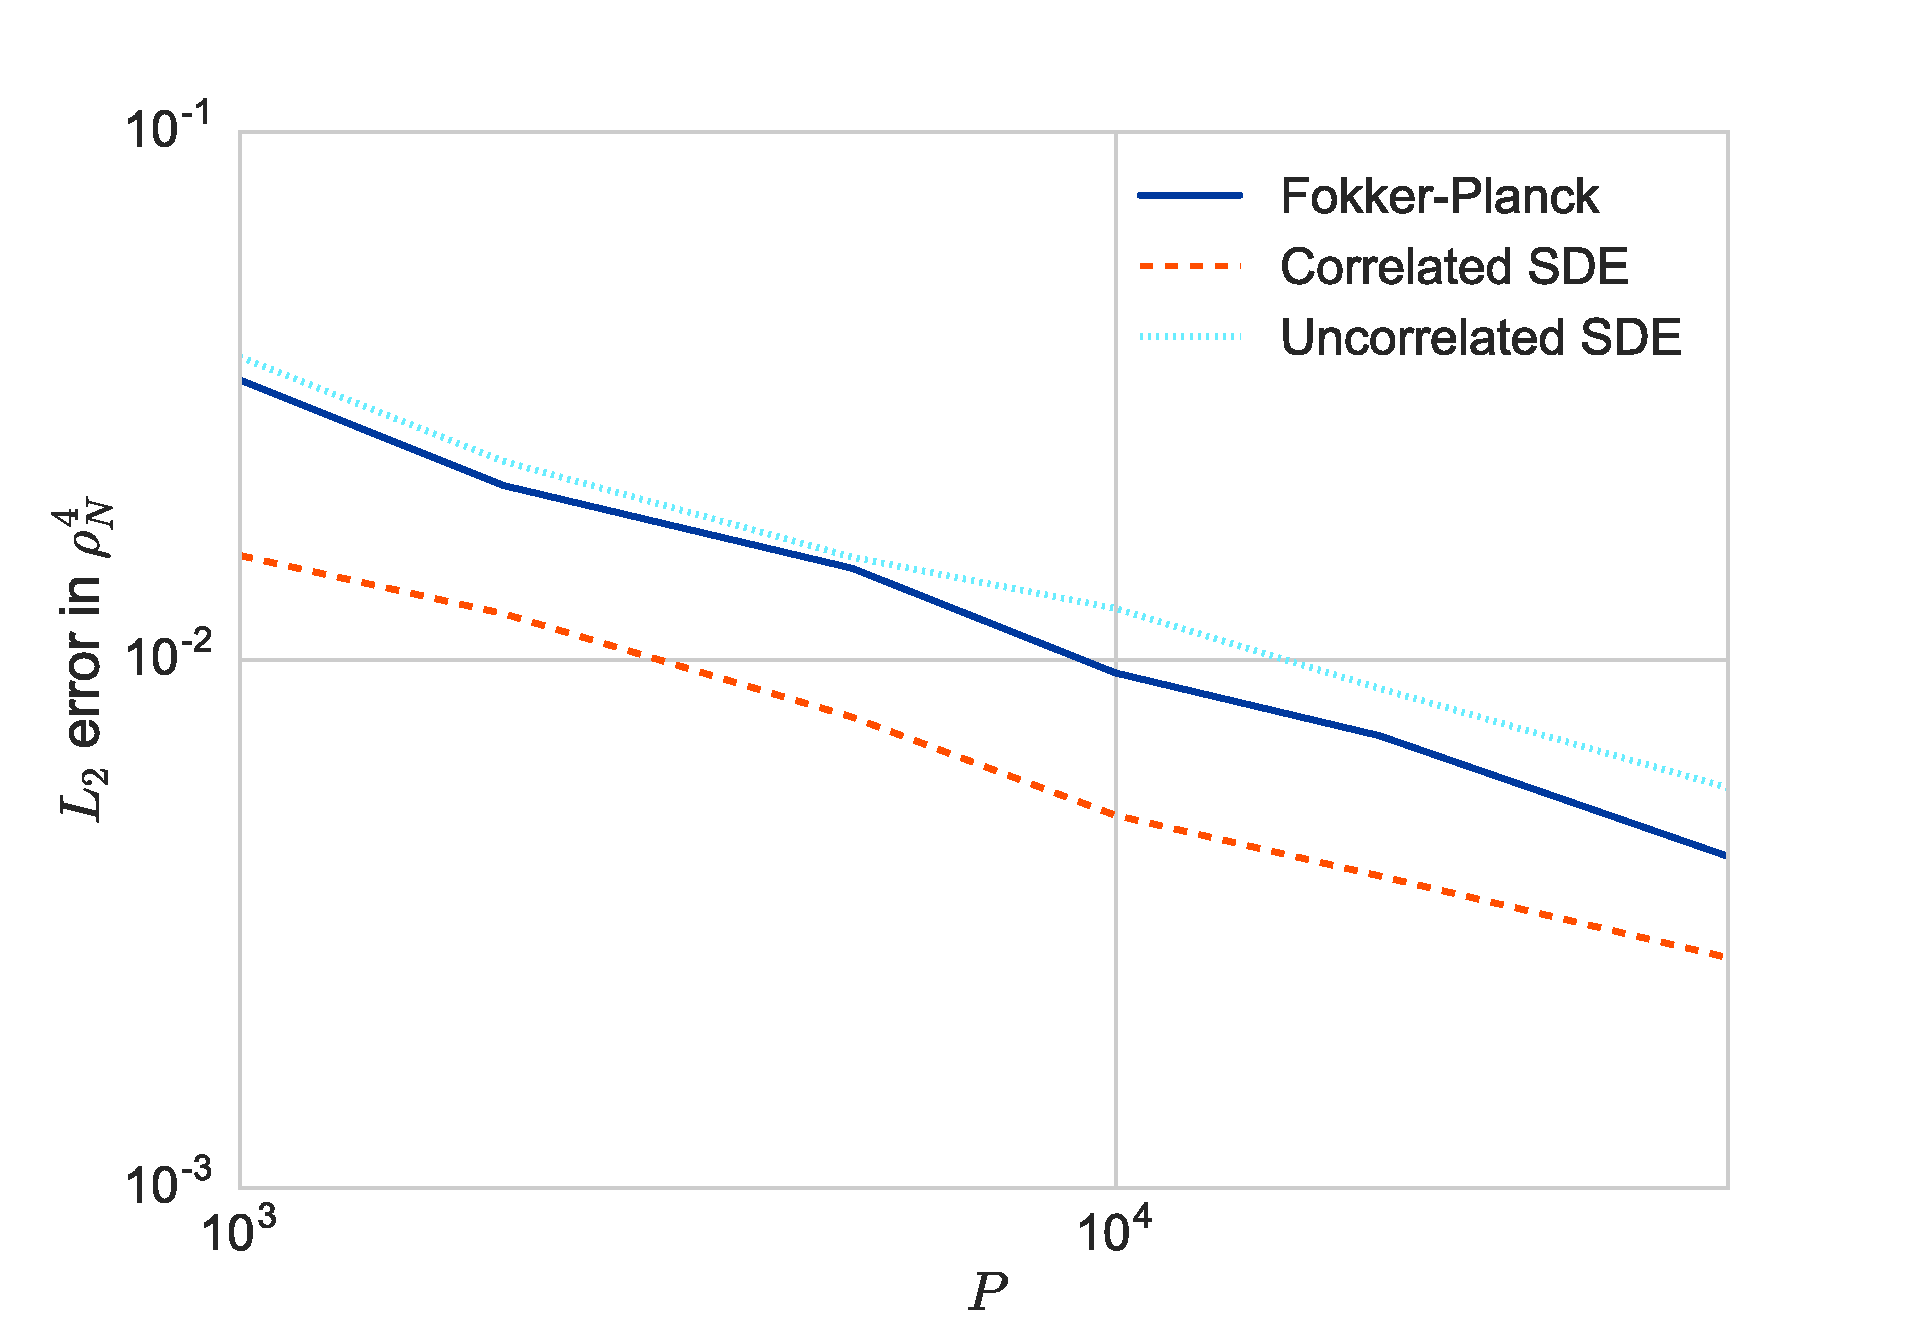
\includegraphics[width=\textwidth]{specific/invalue}
};
\end{tikzpicture}
\end{posterbox}

\begin{posterbox}[name=diagram, column=2, row=0, span=2, textborder=none, headerColorOne=white, headerborder=none]{}
Parameters used below: $\beta=5, \epsilon=0.1, K=N=20, \Delta t = 0.025, \delta t=1.0\times 10^{-4}$
\end{posterbox}

%\begin{posterbox}[name=parameters, column=2, below=notset, above=convergenceK, span=2, textborder=none, headerColorOne=white, headerborder=none]{}
%Parameters used below: $\beta=5, \epsilon=1,N=20,\Delta t = 0.025, \delta t=1.0\times 10^{-4}$
%\end{posterbox}
%
\end{poster}

\end{document}

%%% Local Variables: 
%%% mode: latex
%%% TeX-master: t
%%% End: 
